\subsection{EKF}

前節では、差動二輪ロボットのオドメトリ予測で、向きの不確かさが走行距離に比例して横方向の位置共分散へ伸びることを見た。相補フィルタの固定重みでは、車輪すべり、ジャイロバイアス、外部測定の粗さを時々刻々で区別しにくい。一方、線形 Kalman フィルタの予測共分散、革新、Kalman ゲインは、その区別を数量として持てる。ただし姿勢予測そのものは $\sin\theta$ と $\cos\theta$ を含むため、固定行列 $A,C$ だけでは表せない。したがって次に必要になるのは、平均は非線形なロボット運動学で進め、共分散と革新だけを現在の推定値の近くで線形化する手順である。

線形カルマンフィルタは、線形モデル $A,C$ と共分散 $Q,R$ を使って予測と更新を行った。拡張 Kalman フィルタは、この二段構造を保ったまま、状態遷移と測定の式を非線形写像へ広げる方法である。離散時間の非線形確率モデルを
\begin{align}
  x_k&=f_{k-1}(x_{k-1},u_{k-1})+G_{k-1}w_{k-1},\\
  y_k&=h_k(x_k)+v_k
\end{align}
とする。状態は $x_k\in\R^n$、入力は $u_k\in\R^m$、測定は $y_k\in\R^p$ である。$w_k$ はプロセスノイズ、$v_k$ は測定ノイズであり、
\begin{align}
  E[w_i]&=0,
  &E[v_i]&=0,\\
  E[w_iw_j^\T]&=Q_{w,i}\delta_{ij},
  &E[v_iv_j^\T]&=R_{v,i}\delta_{ij},\\
  E[w_iv_j^\T]&=0
\end{align}
を仮定する。ここで $Q_{w,k}$ は半正定値、$R_{v,k}$ は正定値である。線形カルマンフィルタでは $f(x,u)=Ax+Bu$、$h(x)=Cx$ であった。EKF では、平均値そのものは非線形写像で進め、誤差共分散だけを現在の推定値まわりの一次近似で進める。

予測平均は
\begin{equation}
  \hat{x}_{k|k-1}
  =f_{k-1}(\hat{x}_{k-1|k-1},u_{k-1})
\end{equation}
で与える。状態遷移のヤコビアンを
\begin{equation}
  F_{k-1}
  =
  \left.\frac{\pp f_{k-1}}{\pp x}\right|_{(\hat{x}_{k-1|k-1},u_{k-1})}
\end{equation}
と定義すると、予測誤差 $e_{k|k-1}=x_k-\hat{x}_{k|k-1}$ は一次近似で
\begin{align}
  e_{k|k-1}
  &=f_{k-1}(\hat{x}_{k-1|k-1}+e_{k-1|k-1},u_{k-1})
    -f_{k-1}(\hat{x}_{k-1|k-1},u_{k-1})
    +G_{k-1}w_{k-1}\\
  &\simeq F_{k-1}e_{k-1|k-1}+G_{k-1}w_{k-1}
\end{align}
となる。したがって、交差共分散が 0 であるという仮定から
\begin{equation}
  P_{k|k-1}
  =
  F_{k-1}P_{k-1|k-1}F_{k-1}^\T
  +G_{k-1}Q_{w,k-1}G_{k-1}^\T
\end{equation}
を得る。プロセスノイズが加法的でなく
\begin{equation}
  x_k=f_{k-1}(x_{k-1},u_{k-1},w_{k-1})
\end{equation}
の形で入る場合は、ノイズのヤコビアン
\begin{equation}
  W_{k-1}
  =
  \left.\frac{\pp f_{k-1}}{\pp w}\right|_{(\hat{x}_{k-1|k-1},u_{k-1},0)}
\end{equation}
を用い、上式の $G_{k-1}Q_{w,k-1}G_{k-1}^\T$ を $W_{k-1}Q_{w,k-1}W_{k-1}^\T$ に置き換える。

測定更新では、まず予測測定値を
\begin{equation}
  \hat{y}_{k|k-1}=h_k(\hat{x}_{k|k-1})
\end{equation}
と置き、革新を
\begin{equation}
  \nu_k=y_k-\hat{y}_{k|k-1}
\end{equation}
と定義する。測定写像のヤコビアンは予測状態のまわりで
\begin{equation}
  H_k=
  \left.\frac{\pp h_k}{\pp x}\right|_{\hat{x}_{k|k-1}}
\end{equation}
である。測定式を一次近似すると
\begin{align}
  \nu_k
  &=h_k(x_k)+v_k-h_k(\hat{x}_{k|k-1})\\
  &\simeq H_ke_{k|k-1}+v_k
\end{align}
であるから、革新共分散と Kalman ゲインは
\begin{align}
  S_k&=H_kP_{k|k-1}H_k^\T+R_{v,k},\\
  K_k&=P_{k|k-1}H_k^\T S_k^{-1}
\end{align}
となる。更新後の推定値と共分散は
\begin{align}
  \hat{x}_{k|k}
  &=\hat{x}_{k|k-1}+K_k\nu_k,\\
  P_{k|k}
  &=(I-K_kH_k)P_{k|k-1}(I-K_kH_k)^\T
    +K_kR_{v,k}K_k^\T
\end{align}
である。最後の式は Joseph 形式であり、線形カルマンフィルタと同じ理由で、有限精度計算における対称性と半正定値性を保ちやすい。

\begin{derivation}
EKF の共分散式は、線形カルマンフィルタの式に見た目だけ似せたものではない。状態遷移のテイラー展開
\begin{equation}
  f(\hat{x}+e,u)
  =
  f(\hat{x},u)
  +F e
  +\text{二次以上の項}
\end{equation}
で二次以上の項を無視すると、誤差は $e^-\simeq Fe+Gw$ に従う。したがって
\begin{align}
  P^-
  &=E[e^-(e^-)^\T]\\
  &\simeq E[(Fe+Gw)(Fe+Gw)^\T]\\
  &=F E[ee^\T]F^\T+G E[ww^\T]G^\T
\end{align}
となる。測定側でも $h(\hat{x}^-+e^-)\simeq h(\hat{x}^-)+He^-$ なので、革新は $\nu\simeq He^-+v$ である。この局所線形な革新モデルに対して、線形カルマンフィルタと同じ平均二乗誤差最小化を行うと $K=P^-H^\T(HP^-H^\T+R)^{-1}$ が得られる。
\end{derivation}

$f_{k-1}(x,u)=A_{k-1}x+B_{k-1}u$、$h_k(x)=C_kx$ の場合、ヤコビアンは常に $F_{k-1}=A_{k-1}$、$H_k=C_k$ である。このとき予測平均、共分散、革新、ゲイン、更新の全式は離散時間 Kalman フィルタそのものに戻る。したがって EKF は、線形 Kalman フィルタと別の原理で作られた推定器ではなく、線形 Kalman フィルタを時々刻々の接線モデルへ適用する非線形拡張である。

この解釈は、EKF の限界も同時に示す。一般には $E[f(x)]\ne f(E[x])$ であるため、予測平均を $f(\hat{x})$ で進める操作は厳密な条件付き平均ではない。さらに、共分散は一次テイラー展開に基づくので、推定誤差が大きい、初期値が悪い、測定関数が強く曲がる、ヤコビアンが特異に近い、ノイズが強い非ガウス性を持つ、または角度や姿勢のように状態空間が普通のベクトル空間でない場合には、単一の正規分布と接線モデルだけでは不確かさを十分に表せない。EKF を使うときは、線形化点、サンプリング周期、ノイズ共分散、測定の可観測性を一つの設計条件として確認する必要がある。

\begin{example}[二乗測定をもつスカラー系]
状態がゆっくり変化するスカラー系
\begin{align}
  x_k&=x_{k-1}+w_{k-1},\\
  y_k&=x_k^2+v_k
\end{align}
を考える。状態遷移は線形なので $F_{k-1}=1$、測定写像は $h(x)=x^2$ なので
\begin{equation}
  H_k=\left.\frac{\dd}{\dd x}x^2\right|_{\hat{x}_{k|k-1}}
  =2\hat{x}_{k|k-1}
\end{equation}
である。予測は
\begin{align}
  \hat{x}_{k|k-1}&=\hat{x}_{k-1|k-1},\\
  P_{k|k-1}&=P_{k-1|k-1}+Q_{w,k-1}
\end{align}
となり、革新とゲインは
\begin{align}
  \nu_k&=y_k-\hat{x}_{k|k-1}^2,\\
  S_k&=4\hat{x}_{k|k-1}^2P_{k|k-1}+R_{v,k},\\
  K_k&=\frac{2P_{k|k-1}\hat{x}_{k|k-1}}{S_k}
\end{align}
である。予測値が正で、実測 $y_k$ が予測された二乗値より大きければ、革新は正でゲインも正なので推定値は正方向へ修正される。予測値が負ならゲインの符号も負になり、同じ正の革新は推定値をより負の方向へ修正する。これは、$x^2$ の曲線を現在の予測点で接線近似しているためである。

一方、$\hat{x}_{k|k-1}$ が 0 に近いと $H_k\simeq0$ となり、$K_k$ も小さくなる。測定 $y_k=x_k^2+v_k$ は状態の大きさに関する情報を持つが、符号を区別しない。単一の接線と単一の正規分布で表す EKF は、この大域的な二峰性を表せない。したがって、この例では「非線形測定を線形化して使う」という利点と、「線形化点の周辺でしか情報を正しく読めない」という限界が同時に現れる。
\end{example}

\begin{example}[差動二輪ロボットの外部位置測定による EKF 更新]
オドメトリだけで進む差動二輪ロボットでは、車輪すべりやジャイロバイアスによって経路全体が少しずつ横へずれる。ここに、天井カメラ、測位マーカ、またはランドマーク照合から得られる外部位置測定を時々入れると、非線形予測と線形 Kalman 更新の役割を具体的に見られる。状態を
\begin{equation}
  x_k=
  \begin{bmatrix}
    p_{x,k}\\p_{y,k}\\\theta_k
  \end{bmatrix}
\end{equation}
とし、サンプリング間の走行距離を $\Delta s_k$、向きの変化を $\Delta\theta_k$ とする。予測は、前節のオドメトリと同じく
\begin{align}
  \hat{p}_{x,k|k-1}
  &=
  \hat{p}_{x,k-1|k-1}
  +\Delta s_k\cos\psi_k,\\
  \hat{p}_{y,k|k-1}
  &=
  \hat{p}_{y,k-1|k-1}
  +\Delta s_k\sin\psi_k,\\
  \hat{\theta}_{k|k-1}
  &=
  \hat{\theta}_{k-1|k-1}+\Delta\theta_k,
  \qquad
  \psi_k=\hat{\theta}_{k-1|k-1}+\frac{\Delta\theta_k}{2}
\end{align}
で進める。この式は $\cos\psi_k,\sin\psi_k$ を含むので、平均値は非線形に伝搬する。一方、姿勢誤差が位置誤差へどう移るかは、現在の予測点のヤコビアン
\begin{equation}
  F_k
  =
  \begin{bmatrix}
    1&0&-\Delta s_k\sin\psi_k\\
    0&1& \Delta s_k\cos\psi_k\\
    0&0&1
  \end{bmatrix}
\end{equation}
で共分散へ入る。たとえば前向きに長く走るほど、第三列の大きさが増え、向きの不確かさが横方向の位置不確かさへ写る。

外部測定が位置だけを返す場合を
\begin{equation}
  y_k=
  \begin{bmatrix}
    z_{x,k}\\z_{y,k}
  \end{bmatrix}
  =
  h(x_k)+v_k,
  \qquad
  h(x_k)=
  \begin{bmatrix}
    p_{x,k}\\p_{y,k}
  \end{bmatrix},
  \qquad
  R_k=\sigma_z^2 I
\end{equation}
と書く。予測測定と革新は
\begin{equation}
  \hat{y}_{k|k-1}=
  \begin{bmatrix}
    \hat{p}_{x,k|k-1}\\
    \hat{p}_{y,k|k-1}
  \end{bmatrix},
  \qquad
  \nu_k=
  \begin{bmatrix}
    z_{x,k}-\hat{p}_{x,k|k-1}\\
    z_{y,k}-\hat{p}_{y,k|k-1}
  \end{bmatrix}
\end{equation}
であり、測定ヤコビアンは
\begin{equation}
  H_k=
  \begin{bmatrix}
    1&0&0\\
    0&1&0
  \end{bmatrix}
\end{equation}
である。したがって革新共分散とゲインは
\begin{align}
  S_k
  &=
  H_kP_{k|k-1}H_k^\T+\sigma_z^2I,\\
  K_k
  &=
  P_{k|k-1}H_k^\T S_k^{-1}
  =
  \begin{bmatrix}
    P^-_{xx}&P^-_{xy}\\
    P^-_{yx}&P^-_{yy}\\
    P^-_{\theta x}&P^-_{\theta y}
  \end{bmatrix}
  S_k^{-1}
\end{align}
となる。ここで $P^-_{ij}$ は $P_{k|k-1}$ の成分である。更新は
\begin{align}
  \hat{x}_{k|k}
  &=
  \hat{x}_{k|k-1}+K_k\nu_k,\\
  P_{k|k}
  &=
  (I-K_kH_k)P_{k|k-1}(I-K_kH_k)^\T
  +K_kR_kK_k^\T
\end{align}
である。位置しか測っていなくても、第三行に $P^-_{\theta x},P^-_{\theta y}$ が入るため、予測で生じた位置と向きの相関を通して姿勢も補正される。これは「位置測定から突然角度を測った」わけではなく、非線形オドメトリが作った共分散の傾きを使って、位置ずれを最も起こしやすい向き誤差へ戻しているという解釈である。

測定の信頼度を変えると補正の大きさも変わる。たとえば $x$ 方向だけを見て $P^-_{xx}=0.20^2\,\mathrm{m}^2$ とすると、測定標準偏差が $\sigma_z=0.05\,\mathrm{m}$ のとき
\begin{equation}
  \frac{P^-_{xx}}{P^-_{xx}+\sigma_z^2}
  =
  \frac{0.04}{0.04+0.0025}
  \simeq0.94
\end{equation}
であり、外部測定に近い位置へ強く寄る。測定標準偏差が $\sigma_z=0.50\,\mathrm{m}$ なら
\begin{equation}
  \frac{0.04}{0.04+0.25}
  \simeq0.14
\end{equation}
となり、更新は主にオドメトリ予測を保つ。反対に、すべりを疑ってプロセスノイズを大きくし、$P_{k|k-1}$ を膨らませると、同じ測定でも $K_k$ は大きくなる。したがって $Q$ は「どれだけ予測を疑うか」、$R$ は「どれだけ測定を疑うか」を決める設計量であり、革新 $\nu_k$ が大きすぎるときは $\nu_k^\T S_k^{-1}\nu_k$ を見て外れ値や線形化の破れを疑う。
\end{example}

\subsection{ESKF}

誤差状態 Kalman フィルタ（error-state Kalman filter; ESKF）は、状態そのものを線形化した座標で持つのではなく、非線形な名目状態と、その近くの小さな誤差状態を分けて扱う EKF である。姿勢を四元数 $q$ または回転行列 $R\in\SO(3)$ で表す場合、$q$ には $\norm{q}=1$、$R$ には $R^\T R=I$ と $\det R=1$ という制約がある。通常の EKF のように四元数の 4 成分へ補正量を直接足すと、この制約から外れやすい。足した後に四元数を正規化しても、補正の一部は単位球面の半径方向へ消え、共分散には物理的な姿勢誤差ではない 4 成分目の広がりが残りうる。さらに、補正後の名目姿勢が変わると、その近くの接平面も変わるため、古い座標で持った共分散をそのまま次の時刻へ使うと、局所誤差の意味がずれやすい。ESKF では、姿勢本体は曲面上の名目状態として積分し、共分散は小角度誤差 $\delta\theta\in\R^3$ のような最小座標に持たせる。測定更新で得た小さい誤差を名目状態へ注入し、その直後に誤差平均を 0 へ戻すことで、共分散を常に現在の名目姿勢の接空間に置き直す。

図\ref{fig:flow6-eskf-structure}は、この分離を信号経路として表したものである。IMU 測定は上段の名目状態を多様体上で非線形に伝搬し、同じ測定から下段の誤差状態モデルと共分散伝搬も決まる。外部測定が入ると、名目状態から予測測定を作って革新を計算し、その革新で接空間上の誤差状態を更新する。得られた $\widehat{\delta x}$ は名目状態へ注入され、誤差平均は 0 にリセットされる。この流れにより、姿勢本体は常に $\SO(3)$ または単位四元数上に残り、共分散は名目姿勢の近くの小さい誤差だけを表し続ける。

\begin{figure}[tb]
\centering
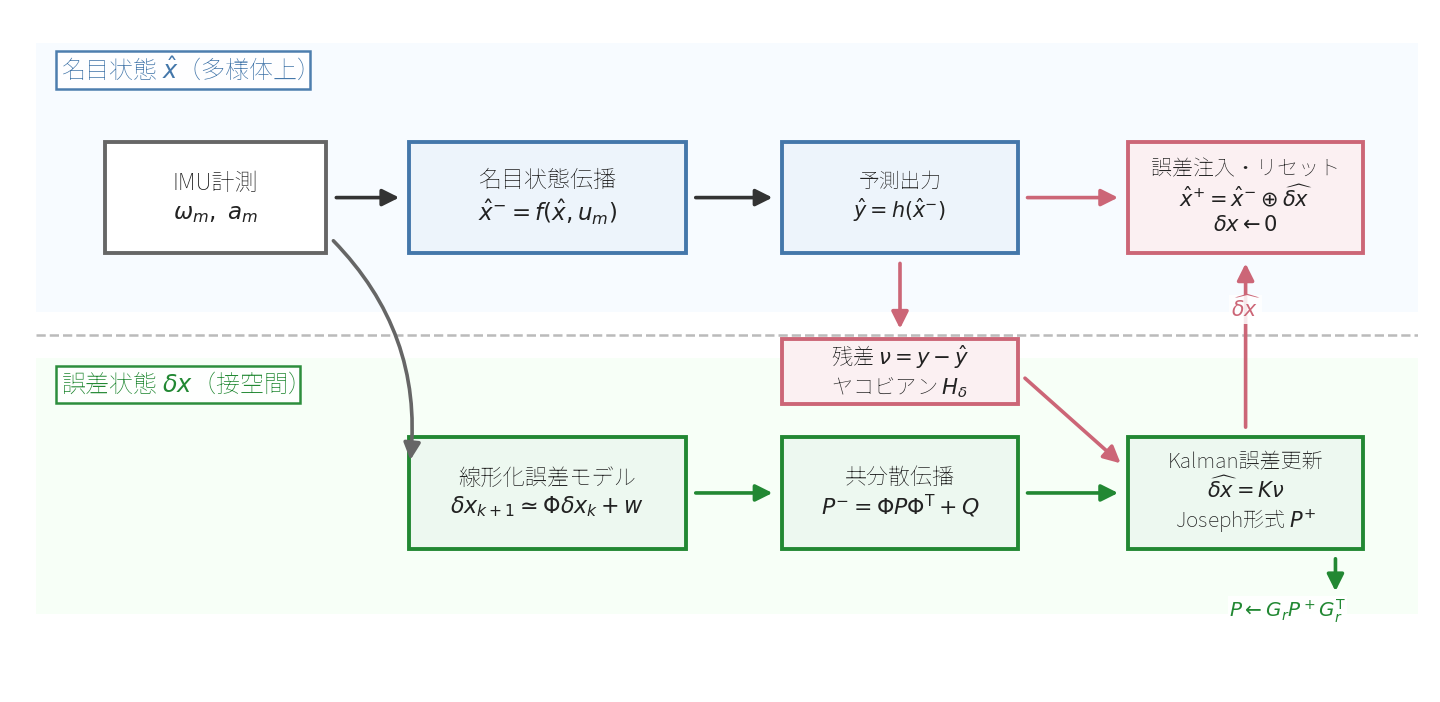
\includegraphics[width=0.96\linewidth,bb=0 0 1440 702]{figures/flow6_eskf_structure.png}
\caption{ESKF における名目状態と誤差状態の分離。IMU 測定は名目状態を伝搬し、同時に接空間上の誤差共分散を伝搬する。測定革新は誤差状態を更新し、推定された誤差は名目状態へ注入されてからリセットされる。}
\label{fig:flow6-eskf-structure}
\end{figure}

\subsubsection{名目状態と誤差状態の分離}

IMU を用いる剛体の推定では、名目状態を
\begin{equation}
  \hat{x}
  =
  \left(
    \hat{p}^I,\hat{v}^I,\hat{q}^I_B,
    \hat{b}_g,\hat{b}_a
  \right)
\end{equation}
のように選ぶことが多い。ここで $\hat{p}^I$ [m] は慣性座標系で表した位置、$\hat{v}^I$ [m/s] は速度、$\hat{q}^I_B$ は機体系 $\{B\}$ から慣性系 $\{I\}$ への姿勢を表す単位四元数、$\hat{b}_g$ [rad/s] はジャイロバイアス、$\hat{b}_a$ [m/s$^2$] は加速度計バイアスである。位置や速度を推定しない姿勢推定では、$p^I,v^I$ を除いた小さい名目状態を使ってもよい。

この名目状態に対応する誤差状態を
\begin{equation}
  \delta x
  =
  \begin{bmatrix}
    \delta p^I\\
    \delta v^I\\
    \delta\theta\\
    \delta b_g\\
    \delta b_a
  \end{bmatrix}
  \in\R^{15}
\end{equation}
と置く。以下で使う $[r]_\times$ は、任意の $s\in\R^3$ に対して $[r]_\times s=r\times s$ を満たす歪対称行列である。真の状態と名目状態の関係は
\begin{align}
  p^I&=\hat{p}^I+\delta p^I,\\
  v^I&=\hat{v}^I+\delta v^I,\\
  q^I_B&=\hat{q}^I_B\otimes\delta q(\delta\theta),\\
  b_g&=\hat{b}_g+\delta b_g,\\
  b_a&=\hat{b}_a+\delta b_a
\end{align}
である。右から掛ける $\delta q(\delta\theta)$ は、名目姿勢から真の姿勢へ戻す小回転を機体系側で表す。小角度では
\begin{equation}
  \delta q(\delta\theta)
  \simeq
  \begin{bmatrix}
    1\\
    \delta\theta/2
  \end{bmatrix}
\end{equation}
であり、回転行列で書けば
\begin{equation}
  R^I_B=\hat{R}^I_B\operatorname{Exp}([\delta\theta]_\times)
  \simeq
  \hat{R}^I_B(I+[\delta\theta]_\times)
\end{equation}
である。したがって、フィルタが持つ共分散 $P$ は四元数 4 成分の共分散ではなく、$\delta p^I,\delta v^I,\delta\theta,\delta b_g,\delta b_a$ に関する共分散である。

IMU の測定モデルを
\begin{align}
  \omega_m&=\omega^B+b_g+n_g,\\
  a_m&=f^B+b_a+n_a
\end{align}
とする。$\omega_m$ [rad/s] はジャイロ測定、$a_m$ [m/s$^2$] は加速度計測定、$\omega^B$ は機体系角速度、$f^B$ は機体系で表した比力である。$n_g,n_a$ は平均 0 の白色ノイズであり、バイアスはゆっくり変わるランダムウォークとして
\begin{align}
  \dot{b}_g&=n_{bg},\\
  \dot{b}_a&=n_{ba}
\end{align}
で表す。比力 $f^B$ は重力を除いた加速度であり、慣性系の重力加速度を $g^I$ とすると並進運動は
\begin{equation}
  \dot{v}^I=R^I_B f^B+g^I
\end{equation}
である。

\subsubsection{連続時間の名目伝搬と誤差伝搬}

名目状態は、IMU 測定からバイアス推定値を引いた
\begin{equation}
  \hat{\omega}=\omega_m-\hat{b}_g,
  \qquad
  \hat{a}=a_m-\hat{b}_a
\end{equation}
を使って非線形に伝搬する。連続時間では
\begin{align}
  \dot{\hat{p}}^I&=\hat{v}^I,\\
  \dot{\hat{v}}^I&=\hat{R}^I_B\hat{a}+g^I,\\
  \dot{\hat{q}}^I_B
  &=
  \frac{1}{2}\hat{q}^I_B\otimes
  \begin{bmatrix}
    0\\ \hat{\omega}
  \end{bmatrix},\\
  \dot{\hat{b}}_g&=0,\\
  \dot{\hat{b}}_a&=0
\end{align}
と書く。数値積分では四元数を随時正規化し、$\norm{\hat{q}^I_B}=1$ を保つ。ここで非線形な姿勢積分そのものを線形モデルへ置き換えているわけではない。線形化するのは、名目状態のまわりの小さな誤差の運動である。

右乗法誤差
\begin{equation}
  R^I_B=\hat{R}^I_B\operatorname{Exp}([\delta\theta]_\times)
\end{equation}
を用い、二次以上の小さい項を無視すると、誤差状態は
\begin{equation}
  \delta\dot{x}
  =
  F_c\delta x+G_cn
\end{equation}
に従う。ただし
\begin{equation}
  n=
  \begin{bmatrix}
    n_g\\ n_a\\ n_{bg}\\ n_{ba}
  \end{bmatrix}
\end{equation}
であり、
\begin{equation}
  F_c=
  \begin{bmatrix}
    0&I&0&0&0\\
    0&0&-\hat{R}^I_B[\hat{a}]_\times&0&-\hat{R}^I_B\\
    0&0&-[\hat{\omega}]_\times&-I&0\\
    0&0&0&0&0\\
    0&0&0&0&0
  \end{bmatrix},
  \qquad
  G_c=
  \begin{bmatrix}
    0&0&0&0\\
    0&-\hat{R}^I_B&0&0\\
    -I&0&0&0\\
    0&0&I&0\\
    0&0&0&I
  \end{bmatrix}.
\end{equation}
第二行の $-\hat{R}^I_B[\hat{a}]_\times\delta\theta$ は、姿勢誤差が比力の慣性系成分を変えることを表す。第三行の $-[\hat{\omega}]_\times\delta\theta-\delta b_g$ は、角速度の名目値まわりで姿勢誤差が回転し、ジャイロバイアス誤差が角度誤差として蓄積することを表す。

\begin{derivation}
速度誤差の主要項は、真の並進式と名目並進式の差から得られる。$a_m-b_a-n_a=\hat{a}-\delta b_a-n_a$ と $R^I_B\simeq\hat{R}^I_B(I+[\delta\theta]_\times)$ を使うと
\begin{align}
  \delta\dot{v}^I
  &=
  R^I_B(a_m-b_a-n_a)-\hat{R}^I_B\hat{a}\\
  &\simeq
  \hat{R}^I_B(I+[\delta\theta]_\times)
  (\hat{a}-\delta b_a-n_a)
  -\hat{R}^I_B\hat{a}\\
  &\simeq
  \hat{R}^I_B[\delta\theta]_\times\hat{a}
  -\hat{R}^I_B\delta b_a
  -\hat{R}^I_B n_a\\
  &=
  -\hat{R}^I_B[\hat{a}]_\times\delta\theta
  -\hat{R}^I_B\delta b_a
  -\hat{R}^I_B n_a .
\end{align}
同様に、姿勢の右誤差を一次まで残すと
\begin{equation}
  \delta\dot{\theta}
  \simeq
  -[\hat{\omega}]_\times\delta\theta-\delta b_g-n_g
\end{equation}
となる。
\end{derivation}

\subsubsection{離散時間予測と共分散伝搬}

サンプリング周期を $\Delta t$ とする。もっとも単純な一段の離散化では、名目状態を
\begin{align}
  \hat{p}^I_{k+1}
  &=
  \hat{p}^I_k+\hat{v}^I_k\Delta t
  +\frac{1}{2}(\hat{R}^I_{B,k}\hat{a}_k+g^I)\Delta t^2,\\
  \hat{v}^I_{k+1}
  &=
  \hat{v}^I_k+(\hat{R}^I_{B,k}\hat{a}_k+g^I)\Delta t,\\
  \hat{q}^I_{B,k+1}
  &=
  \hat{q}^I_{B,k}\otimes\delta q(\hat{\omega}_k\Delta t),\\
  \hat{b}_{g,k+1}&=\hat{b}_{g,k},\\
  \hat{b}_{a,k+1}&=\hat{b}_{a,k}
\end{align}
で進める。実装では、姿勢更新後に
\begin{equation}
  \hat{q}^I_{B,k+1}
  \leftarrow
  \frac{\hat{q}^I_{B,k+1}}{\norm{\hat{q}^I_{B,k+1}}}
\end{equation}
と正規化する。高精度が必要なら、中点法や Runge--Kutta 法で名目状態を積分し、同じ区間で誤差遷移行列も積分する。

誤差状態の離散近似は
\begin{equation}
  \delta x_{k+1}
  \simeq
  \Phi_k\delta x_k+w_{\delta,k}
\end{equation}
であり、一次近似では
\begin{equation}
  \Phi_k\simeq I+F_{c,k}\Delta t
\end{equation}
である。連続時間白色ノイズの共分散密度を
\begin{equation}
  E[n(t)n(\tau)^\T]=Q_c\delta(t-\tau)
\end{equation}
で定義すると、離散時間のプロセスノイズ共分散は
\begin{equation}
  Q_{d,k}
  =
  \int_0^{\Delta t}
  \Phi(\Delta t-\tau)G_cQ_cG_c^\T
  \Phi(\Delta t-\tau)^\T\,\dd\tau
\end{equation}
で定義される。短い周期では
\begin{equation}
  Q_{d,k}\simeq G_{c,k}Q_cG_{c,k}^\T\Delta t
\end{equation}
を用いることが多い。したがって共分散予測は
\begin{equation}
  P_{k+1|k}
  =
  \Phi_kP_{k|k}\Phi_k^\T+Q_{d,k}
\end{equation}
である。

\subsubsection{測定更新と誤差注入}

位置、速度、姿勢、重力方向、磁気方位、距離などの測定をまとめて
\begin{equation}
  y_k=h(\hat{x}_{k|k-1}\oplus\delta x_k)+v_k
\end{equation}
と書く。記号 $\oplus$ は、ユークリッド成分には足し算、姿勢成分には小回転の乗法を使って誤差を名目状態へ載せる操作を表す。測定の予測値と革新を
\begin{equation}
  \hat{y}_{k|k-1}=h(\hat{x}_{k|k-1}),
  \qquad
  \nu_k=y_k-\hat{y}_{k|k-1}
\end{equation}
と置き、誤差状態に関する測定ヤコビアンを
\begin{equation}
  H_{\delta,k}
  =
  \left.
  \frac{\pp h(\hat{x}_{k|k-1}\oplus\delta x)}
       {\pp\delta x}
  \right|_{\delta x=0}
\end{equation}
で定義する。一次近似では
\begin{equation}
  \nu_k\simeq H_{\delta,k}\delta x_k+v_k
\end{equation}
となるので、通常の Kalman 型更新として
\begin{align}
  S_k&=H_{\delta,k}P_{k|k-1}H_{\delta,k}^\T+R_k,\\
  K_k&=P_{k|k-1}H_{\delta,k}^\T S_k^{-1},\\
  \widehat{\delta x}_k&=K_k\nu_k,\\
  P^+_k
  &=(I-K_kH_{\delta,k})P_{k|k-1}
    (I-K_kH_{\delta,k})^\T+K_kR_kK_k^\T
\end{align}
を計算する。ここで $\widehat{\delta x}_k$ は、真の誤差状態の推定値である。

更新後は、推定された誤差を名目状態へ注入し、誤差状態の平均を 0 に戻す。すなわち
\begin{align}
  \hat{p}^{I,+}&=\hat{p}^{I,-}+\widehat{\delta p}^I,\\
  \hat{v}^{I,+}&=\hat{v}^{I,-}+\widehat{\delta v}^I,\\
  \hat{q}^{I,+}_B
  &=
  \hat{q}^{I,-}_B\otimes
  \delta q(\widehat{\delta\theta}),\\
  \hat{b}^+_g&=\hat{b}^-_g+\widehat{\delta b}_g,\\
  \hat{b}^+_a&=\hat{b}^-_a+\widehat{\delta b}_a
\end{align}
とし、四元数を正規化する。続いて
\begin{equation}
  \delta x\leftarrow0
\end{equation}
とリセットする。このリセットは平均だけでなく共分散にも影響する。注入前の誤差から注入後の誤差への一次変換を $G_r$ とすれば
\begin{equation}
  P_{k|k}=G_rP^+_kG_r^\T
\end{equation}
である。右乗法の小さい姿勢補正では、姿勢ブロックに
\begin{equation}
  G_{r,\theta\theta}
  \simeq
  I-\frac{1}{2}[\widehat{\delta\theta}]_\times
\end{equation}
を使うことが多い。補正角が十分小さい場合は $G_r\simeq I$ としても大きな差は出にくいが、大きな革新を頻繁に注入する実装では、リセットヤコビアンを省くと共分散の整合性が悪くなる。

\subsubsection{ESKF の数値トレース}

式だけでは、名目姿勢と誤差状態を分ける利点を数量として追いにくい。ここでは、ピッチ角だけを取り出した 1 次元の姿勢更新で、IMU 予測、共分散、革新、注入、リセットを数値で追う。ジャイロ積分だけで進む名目角は、未補償のジャイロバイアスによって少しずつ真値から離れる。一方、加速度計から得る傾きは重力方向を使うため低速時にはロールとピッチを拘束できるが、並進加速度が混ざると重力方向そのものからずれる。この二つの限界を、ESKF は「予測をどれだけ疑うか」を $P^-_{\theta,k}$、「加速度計の傾きをどれだけ信じるか」を $R_{\theta,k}$ として分けて扱う。

数値例では、時刻 $t=4.0\,\mathrm{s}$ で真のピッチ角が $0.55^\circ$、ジャイロ積分で得た名目予測が $1.56^\circ$、加速度計から作った傾き測定が $-0.20^\circ$ であったとする。このとき革新は
\begin{equation}
  \nu_{\theta,k}
  =
  y_{\theta,k}-\hat{\theta}^{-}_k
  =
  -1.76^\circ
\end{equation}
であり、更新直前の姿勢標準偏差は $\sqrt{P^-_{\theta,k}}=1.52^\circ$ まで増えている。ピッチだけに限定すると、誤差状態の測定モデルは
\begin{equation}
  \nu_{\theta,k}
  \simeq
  \delta\theta_k+v_{\theta,k}
\end{equation}
なので
\begin{align}
  S_{\theta,k}&=P^-_{\theta,k}+R_{\theta,k},\\
  K_{\theta,k}&=P^-_{\theta,k}S_{\theta,k}^{-1},\\
  \widehat{\delta\theta}_k&=K_{\theta,k}\nu_{\theta,k},\\
  P^+_{\theta,k}
  &=(1-K_{\theta,k})^2P^-_{\theta,k}
    +K_{\theta,k}^2R_{\theta,k}
\end{align}
で更新できる。たとえば加速度計の傾き標準偏差を $1.20^\circ$ と仮定する標準設定では、$K_{\theta,k}=0.62$、$\widehat{\delta\theta}_k=-1.09^\circ$、$\sqrt{P^+_{\theta,k}}=0.94^\circ$ となる。この小角度を名目姿勢へ
\begin{equation}
  \hat{q}^{+}
  =
  \hat{q}^{-}\otimes\delta q(\widehat{\delta\theta}_k)
\end{equation}
として注入し、直後に誤差平均を
\begin{equation}
  \delta\theta\leftarrow0
\end{equation}
へ戻す。今回の 1 次元トレースでは補正角が小さいため $G_{r,\theta\theta}\simeq1$ と近似し、共分散はほぼ $P^+_{\theta,k}$ のまま現在の名目姿勢まわりの誤差幅として読み替えられる。

\begin{figure}[tb]
\centering
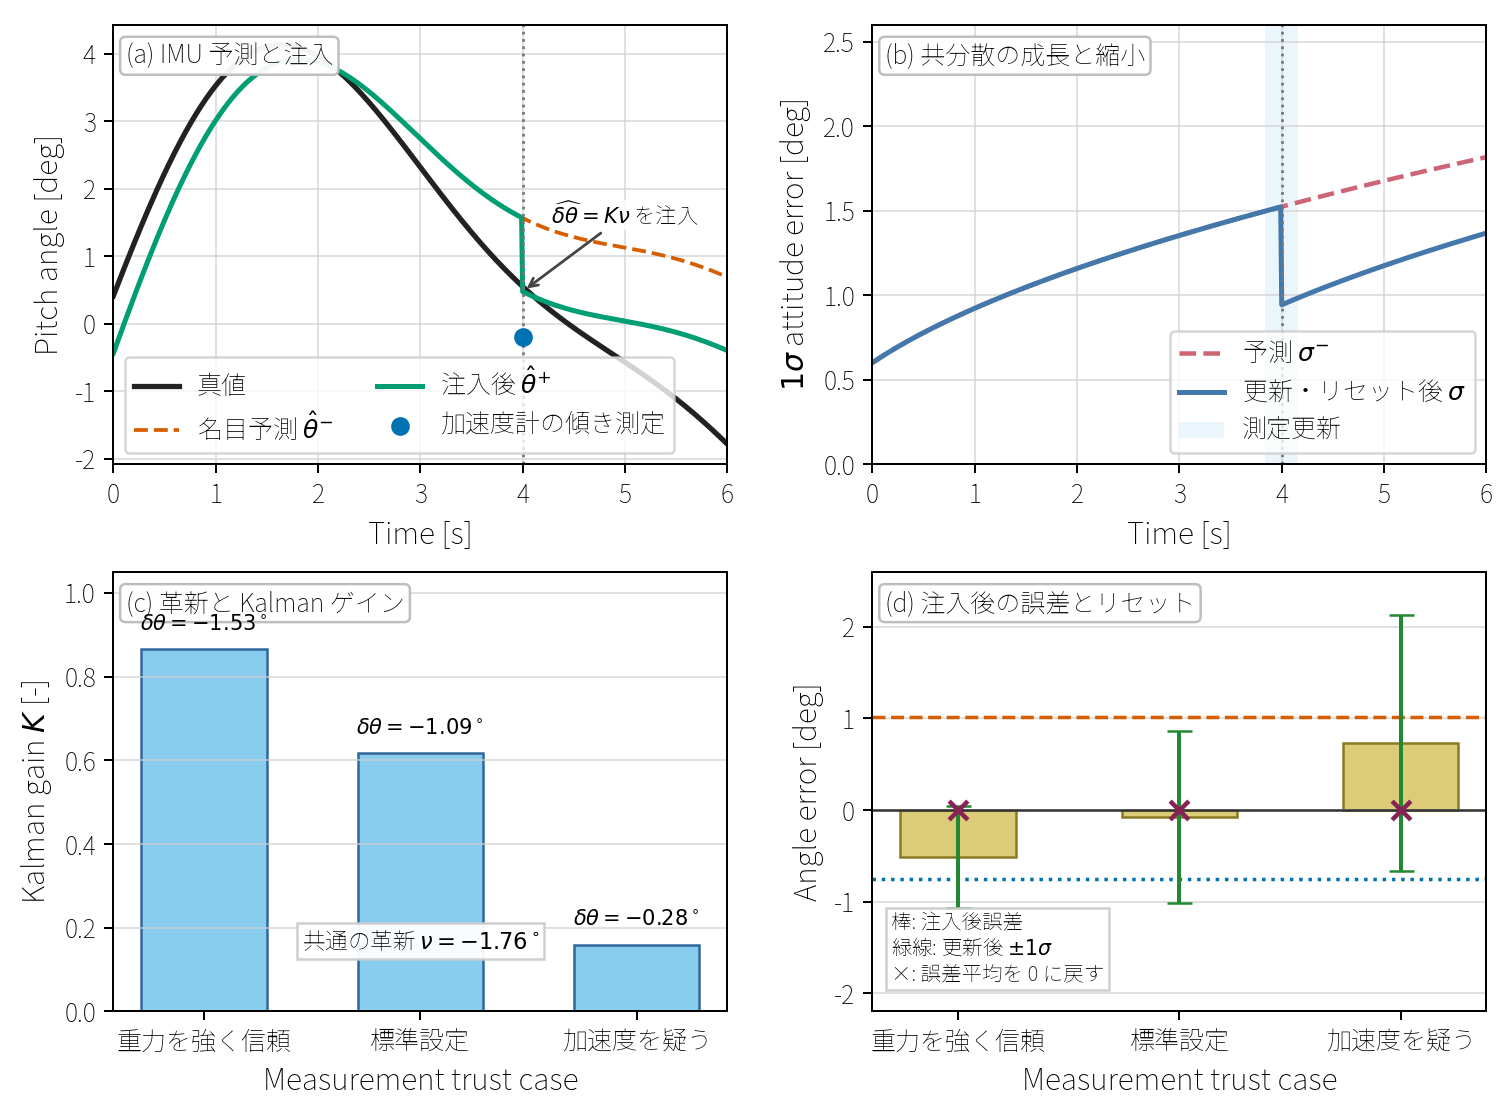
\includegraphics[width=0.98\linewidth,bb=0 0 1512 1116]{figures/flow6_eskf_numeric_trace.png}
\caption{ESKF の 1 次元姿勢更新トレース。ジャイロ積分で名目姿勢がドリフトし、同時に姿勢共分散が増える。加速度計から得た傾き測定の革新で小角度誤差 $\widehat{\delta\theta}$ を推定し、名目姿勢へ注入してから誤差平均を 0 へリセットする。測定を強く信頼すると加速度外乱にも寄りやすく、測定を疑うとジャイロドリフトが残りやすい。}
\label{fig:flow6-eskf-numeric-trace}
\end{figure}

図\ref{fig:flow6-eskf-numeric-trace}では、上段左に真値、ジャイロ積分だけの名目予測、注入後の名目姿勢を重ねている。上段右では、更新前の標準偏差が時間とともに増え、測定更新で小さくなった後、再びジャイロノイズとバイアス不確かさで増える。下段左は測定信頼度を変えたときの Kalman ゲインであり、加速度計を強く信頼する $0.60^\circ$ 設定では $K=0.87$、標準設定では $K=0.62$、急加速中として疑う $3.50^\circ$ 設定では $K=0.16$ になる。同じ革新 $-1.76^\circ$ でも、注入する局所姿勢誤差はそれぞれ $-1.53^\circ$、$-1.09^\circ$、$-0.28^\circ$ に変わる。

下段右は、この重み付けが破綻モードの解釈を決めることを示している。加速度計を強く信頼すると、ジャイロドリフトによる $1.01^\circ$ の予測誤差は大きく消えるが、加速度計の傾きに $-0.75^\circ$ の非重力加速度成分が混ざっていると、その外乱にも引かれる。反対に加速度計を強く疑うと、外乱には引かれにくいが、更新後も正の姿勢誤差が残る。したがって、静止または低加速度で重力方向が信頼できる時刻は $R_{\theta,k}$ を小さくでき、急加速、振動、衝突、センサ飽和が疑われる時刻は $R_{\theta,k}$ を大きくするか革新を棄却する必要がある。重力方向だけではヨー角を拘束できないため、ヨーのジャイロドリフトには磁気方位、外部姿勢、位置変化から得た方位情報など、別の測定が必要になる。

\subsubsection{EKF との関係と適用条件}

ESKF は EKF と別のベイズ更新を使う方法ではない。予測、革新、Kalman ゲイン、Joseph 形式の共分散更新は EKF と同じであり、違いは線形化する座標である。通常の EKF は状態 $x$ の足し算
\begin{equation}
  x=\hat{x}+\delta x
\end{equation}
を前提にする。一方、ESKF は
\begin{equation}
  x=\hat{x}\oplus\delta x
\end{equation}
を用い、姿勢のような多様体上の成分だけを乗法的に扱う。すべての状態がユークリッド空間にあり、$\oplus$ が普通の足し算である場合、ESKF の式は EKF の誤差座標表示に戻る。

ESKF が有効に働くには、注入とリセットによって誤差状態が小さい領域に保たれること、IMU のサンプリング周期が姿勢変化に対して十分短いこと、ノイズ共分散とバイアスランダムウォークの大きさが現実的に設定されていること、測定モデルの可観測性が確保されていることが必要である。加速度計だけでは重力方向からロールとピッチを拘束できるが、ヨー角は拘束できない。磁気センサや外部位置センサを使う場合も、磁気外乱、加速度計の非重力加速度、センサ飽和、時刻同期ずれ、座標系の取り違えがあると、革新が小角度誤差の仮定を破りやすい。初期姿勢が大きく外れている場合は、ESKF の局所線形更新へ入る前に粗い初期合わせを行うか、大きな不確かさを表せる別の初期化手順を用いる。

\begin{example}[重力方向を使う姿勢 IMU の ESKF]
位置と速度を使わず、姿勢、ジャイロバイアス、加速度計バイアスだけを推定する例を考える。名目状態は
\begin{equation}
  \hat{x}=(\hat{q}^I_B,\hat{b}_g,\hat{b}_a)
\end{equation}
であり、誤差状態は
\begin{equation}
  \delta x=
  \begin{bmatrix}
    \delta\theta\\
    \delta b_g\\
    \delta b_a
  \end{bmatrix}
  \in\R^9
\end{equation}
である。ジャイロで姿勢を
\begin{equation}
  \hat{q}^I_{B,k+1}
  =
  \hat{q}^I_{B,k}\otimes
  \delta q\left((\omega_{m,k}-\hat{b}_{g,k})\Delta t\right)
\end{equation}
と予測する。低加速度で、加速度計がほぼ重力方向だけを測っていると仮定できる時刻には、
\begin{equation}
  y_k=a_{m,k}
  \simeq
  -(\hat{R}^I_{B,k})^\T g^I+\hat{b}_{a,k}+v_k
\end{equation}
を測定モデルとして使える。ここで $g^I=\begin{bmatrix}0&0&-g\end{bmatrix}^\T$ である。誤差状態に関する一次近似は
\begin{equation}
  \nu_k
  =
  a_{m,k}
  +(\hat{R}^I_{B,k})^\T g^I-\hat{b}_{a,k}
  \simeq
  H_{\delta,k}\delta x_k+v_k
\end{equation}
であり、
\begin{equation}
  H_{\delta,k}
  =
  \begin{bmatrix}
    -[(\hat{R}^I_{B,k})^\T g^I]_\times
    &0&I
  \end{bmatrix}
\end{equation}
である。この更新は、重力方向と一致するようにロール角とピッチ角を補正し、加速度計バイアスに対する革新も作る。ただし、静止に近い重力測定だけでは、小さな傾きと加速度計バイアスが強く結合する。一方、重力ベクトルのまわりの回転であるヨー角はこの測定だけでは観測できない。したがって、ヨー角とバイアスを長時間安定させるには、磁気方位、外部姿勢、位置変化から得られる方位情報など、重力以外の測定が必要になる。
\end{example}

\subsection{誤差状態と力学座標の接続整理}

ESKF までの議論では、非線形状態をそのまま線形ベクトルとして扱わず、名目状態と小さな誤差を分けることで、推定の共分散を接空間上に置いた。ここではその考え方を、座標変換、姿勢表現、エネルギーに基づく力学モデルへ戻して整理する。以下の接線モデルは EKF/ESKF が何を線形化しているかの確認であり、小角度四元数とオイラー・ラグランジュ方程式は、同じ非線形対象を局所誤差座標または一般化座標で扱うための橋渡しである。

\begin{definition}[接線モデル]
非線形写像 $f(x,u)$ を現在の点 $(\bar{x},\bar{u})$ の近くで一次テイラー展開した
\begin{equation}
  f(x,u)\simeq f(\bar{x},\bar{u})+F(x-\bar{x})+G(u-\bar{u})
\end{equation}
を接線モデルという。ただし
\begin{equation}
  F=\left.\frac{\pp f}{\pp x}\right|_{(\bar{x},\bar{u})},
  \qquad
  G=\left.\frac{\pp f}{\pp u}\right|_{(\bar{x},\bar{u})}
\end{equation}
である。
\end{definition}

EKF で行っていることは、非線形モデルを捨てることではない。予測そのものは
\begin{equation}
  \hat{x}_{k+1|k}=f(\hat{x}_{k|k},u_k)
\end{equation}
で非線形に進める。一方、共分散は「小さな誤差がどう伝わるか」を見るので、誤差 $\delta x_k=x_k-\hat{x}_{k|k}$ を用いて
\begin{align}
  x_{k+1}-\hat{x}_{k+1|k}
  &=f(\hat{x}_{k|k}+\delta x_k,u_k)-f(\hat{x}_{k|k},u_k)\\
  &\simeq F_k\delta x_k
\end{align}
と近似する。したがって
\begin{equation}
  P_{k+1|k}=F_kP_{k|k}F_k^\T+Q
\end{equation}
になる。

三次元姿勢は特殊直交群 $\SO(3)$ の元であり、通常のベクトル空間ではない。回転行列 $R$ に小さな行列を単純に足すと、一般には $R^\T R=I$ が壊れる。四元数でも単位制約 $\norm{q}=1$ を保つ必要がある。したがって ESKF の姿勢更新は、状態成分へ直接補正を足す操作ではなく、小さな誤差を接空間で表してから回転へ戻す操作として解釈する。

\begin{formula}[小角度四元数の局所誤差表示]
小さな回転ベクトル $\delta\theta\in\R^3$ に対応する四元数は一次近似で
\begin{equation}
  \delta q\simeq
  \begin{bmatrix}1\\ \delta\theta/2\end{bmatrix}
\end{equation}
である。
\end{formula}

\begin{derivation}
回転軸 $a$、角度 $\alpha$ の四元数は
\begin{equation}
  q=\begin{bmatrix}\cos(\alpha/2)\\ a\sin(\alpha/2)\end{bmatrix}
\end{equation}
である。小角度ではテイラー展開より
\begin{equation}
  \cos(\alpha/2)\simeq1,
  \qquad
  \sin(\alpha/2)\simeq\alpha/2.
\end{equation}
また $\delta\theta=a\alpha$ なので
\begin{equation}
  a\sin(\alpha/2)\simeq a\alpha/2=\delta\theta/2
\end{equation}
となり、小角度四元数の式を得る。
\end{derivation}

ESKF の姿勢更新
\begin{equation}
  \hat{q}^{+}=\hat{q}^{-}\otimes\delta q(\widehat{\delta\theta})
\end{equation}
では、$\widehat{\delta\theta}$ は推定された小回転誤差であり、更新時に名目姿勢へ注入された直後に平均 0 の誤差状態へ戻される。したがって共分散を持つ座標は、四元数の 4 成分そのものではなく、注入前後の接空間に置かれた $\delta\theta$ の 3 成分である。リセット後の共分散は、必要に応じて $G_rP^+G_r^\T$ により新しい接空間へ写される。

これに対して単振子の記述で $\theta=\hat{\theta}+\delta\theta$ と書くとき、$\theta$ は
\begin{equation}
  T=\frac{1}{2}m\ell^2\dot{\theta}^2,\qquad
  U=mg\ell(1-\cos\theta)
\end{equation}
を立てる一般化座標である。線形化では
\begin{equation}
  \sin(\hat{\theta}+\delta\theta)
  \simeq
  \sin\hat{\theta}+\cos\hat{\theta}\,\delta\theta
\end{equation}
のように、固定した名目値 $\hat{\theta}$ のまわりで小さい変化 $\delta\theta$ だけを一次まで残す。したがって、ESKF では共分散の座標が接空間の誤差 $\delta\theta$、力学式を立てる座標が実姿勢または一般化座標 $\theta$、線形化点として固定される値が名目状態 $\hat{\theta}$ または $\hat{q}$ である。この三者の分離が、姿勢推定の局所誤差と力学モデルの一般化座標を接続する条件になる。

この区別を保つと、姿勢推定で使う局所誤差と、機械系の運動方程式で使う一般化座標を同じ記号の引き算として混同しにくくなる。最後に、エネルギーから運動方程式を得る定式化として、オイラー・ラグランジュ方程式を接続用に再掲する。

\begin{theorem}[オイラー・ラグランジュ方程式]
作用積分 $S=\int_{t_0}^{t_1}L(q,\dot{q},t)\,\dd t$ が、端点固定の微小変分に対して停留値をとるなら
\begin{equation}
  \frac{\dd}{\dd t}\frac{\pp L}{\pp\dot{q}_i}-\frac{\pp L}{\pp q_i}=0
\end{equation}
が成り立つ。非保存力が一般化力 $Q_i$ として入ると右辺は $Q_i$ になる。
\end{theorem}

この定理は、力を一つずつ座標軸へ分解する代わりに、エネルギーから運動方程式を得るための定式化である。単振子の導出では、$L=T-V$ を書き、$\pp L/\pp\dot{\theta}$、$\pp L/\pp\theta$ を実際に計算して代入している。

\subsection{UKF と粒子フィルタによる非線形ベイズ推定}

EKF は非線形写像を接線で近似する。これに対して、Unscented Kalman フィルタ（UKF）は、分布を代表する少数の点を非線形写像へ通し、その通過後の平均と共分散を計算する。さらに粒子フィルタは、平均と共分散だけでなく、事後分布そのものを重み付きサンプルの集合で近似する。三つの方法はいずれも、ベイズフィルタの予測
\begin{equation}
  p(x_k\mid y_{1:k-1})
  =
  \int p(x_k\mid x_{k-1},u_{k-1})
  p(x_{k-1}\mid y_{1:k-1})\,\dd x_{k-1}
\end{equation}
と更新
\begin{equation}
  p(x_k\mid y_{1:k})
  =
  \frac{p(y_k\mid x_k)p(x_k\mid y_{1:k-1})}
       {p(y_k\mid y_{1:k-1})}
\end{equation}
を近似する方法である。違いは、事後分布を単一の正規分布と接線で表すか、シグマ点で表すか、粒子集合で表すかにある。

\begin{definition}[Unscented 変換とシグマ点]
平均 $\bar{x}\in\R^n$、共分散 $P=P^\T\ge0$ をもつ確率変数 $x$ を、非線形写像 $z=g(x)$ へ通すことを考える。UKF ではまず
\begin{equation}
  \lambda=\alpha^2(n+\kappa)-n
\end{equation}
を定め、行列平方根 $S$ を
\begin{equation}
  SS^\T=(n+\lambda)P
\end{equation}
で選ぶ。$S_{:i}$ を $S$ の第 $i$ 列とすると、$2n+1$ 個のシグマ点を
\begin{align}
  \chi^{(0)}&=\bar{x},\\
  \chi^{(i)}&=\bar{x}+S_{:i}\qquad(i=1,\ldots,n),\\
  \chi^{(i+n)}&=\bar{x}-S_{:i}\qquad(i=1,\ldots,n)
\end{align}
と置く。重みは
\begin{align}
  W_m^{(0)}&=\frac{\lambda}{n+\lambda},\\
  W_c^{(0)}&=\frac{\lambda}{n+\lambda}+1-\alpha^2+\beta,\\
  W_m^{(i)}&=W_c^{(i)}=\frac{1}{2(n+\lambda)}
  \qquad(i=1,\ldots,2n)
\end{align}
である。ここで $\alpha$ はシグマ点の広がり、$\kappa$ は補助的なスケール、$\beta$ は事前分布の形に関する調整量である。
\end{definition}

各シグマ点を
\begin{equation}
  \zeta^{(i)}=g(\chi^{(i)})
\end{equation}
で写像した後、出力側の平均と共分散を
\begin{align}
  \bar{z}
  &\simeq \sum_{i=0}^{2n}W_m^{(i)}\zeta^{(i)},\\
  P_z
  &\simeq \sum_{i=0}^{2n}W_c^{(i)}
  \left(\zeta^{(i)}-\bar{z}\right)
  \left(\zeta^{(i)}-\bar{z}\right)^\T
\end{align}
で近似する。この操作を Unscented 変換という。シグマ点はもとの平均と共分散を再現するように置かれているので、非線形写像の曲がりを、ヤコビアンを計算せずに平均と共分散へ反映できる。ただし、UKF も最終的には単一の平均と共分散に戻すため、多峰性や強い非ガウス性をそのまま保持する方法ではない。

UKF の予測は、EKF と同じ非線形確率モデル
\begin{align}
  x_k&=f_{k-1}(x_{k-1},u_{k-1})+w_{k-1},\\
  y_k&=h_k(x_k)+v_k
\end{align}
を仮定して書ける。$w_{k-1}$ と $v_k$ は平均 0、共分散 $Q_{k-1}$、$R_k$ をもつ加法ノイズとする。時刻 $k-1$ の推定値 $\hat{x}_{k-1|k-1}$、共分散 $P_{k-1|k-1}$ からシグマ点 $\chi_{k-1|k-1}^{(i)}$ を作り、
\begin{equation}
  \chi_{k|k-1}^{(i)}
  =
  f_{k-1}(\chi_{k-1|k-1}^{(i)},u_{k-1})
\end{equation}
で伝搬する。予測平均と予測共分散は
\begin{align}
  \hat{x}_{k|k-1}
  &=\sum_{i=0}^{2n}W_m^{(i)}\chi_{k|k-1}^{(i)},\\
  P_{k|k-1}
  &=\sum_{i=0}^{2n}W_c^{(i)}
  \left(\chi_{k|k-1}^{(i)}-\hat{x}_{k|k-1}\right)
  \left(\chi_{k|k-1}^{(i)}-\hat{x}_{k|k-1}\right)^\T
  +Q_{k-1}
\end{align}
である。ノイズが加法的でない場合は、状態とノイズを合わせた拡大状態に対してシグマ点を作り、同じ考え方で伝搬する。

測定更新では、予測シグマ点を測定写像へ通して
\begin{equation}
  \gamma_k^{(i)}=h_k(\chi_{k|k-1}^{(i)})
\end{equation}
とし、予測測定、革新共分散、状態と測定の交差共分散を
\begin{align}
  \hat{y}_{k|k-1}
  &=\sum_{i=0}^{2n}W_m^{(i)}\gamma_k^{(i)},\\
  S_k
  &=\sum_{i=0}^{2n}W_c^{(i)}
  \left(\gamma_k^{(i)}-\hat{y}_{k|k-1}\right)
  \left(\gamma_k^{(i)}-\hat{y}_{k|k-1}\right)^\T
  +R_k,\\
  C_k
  &=\sum_{i=0}^{2n}W_c^{(i)}
  \left(\chi_{k|k-1}^{(i)}-\hat{x}_{k|k-1}\right)
  \left(\gamma_k^{(i)}-\hat{y}_{k|k-1}\right)^\T
\end{align}
で計算する。Kalman ゲインと更新式は
\begin{align}
  K_k&=C_kS_k^{-1},\\
  \hat{x}_{k|k}
  &=\hat{x}_{k|k-1}+K_k(y_k-\hat{y}_{k|k-1}),\\
  P_{k|k}
  &=P_{k|k-1}-K_kS_kK_k^\T
\end{align}
である。EKF では $F_k,H_k$ というヤコビアンを作ってから線形 Kalman フィルタへ戻るが、UKF では $2n+1$ 個の点を実際に $f,h$ へ通してから Kalman 型の更新へ戻る。

粒子フィルタでは、事後分布を
\begin{equation}
  p(x_k\mid y_{1:k})
  \simeq
  \sum_{i=1}^{N}W_k^{(i)}\delta(x_k-x_k^{(i)})
\end{equation}
のように、粒子 $x_k^{(i)}$ と正規化重み $W_k^{(i)}$ の集合で表す。ここで
\begin{equation}
  W_k^{(i)}\ge0,\qquad
  \sum_{i=1}^{N}W_k^{(i)}=1
\end{equation}
であり、$\delta$ は一点に質量を置く Dirac のデルタである。この近似のもとで、任意の関数 $\varphi(x)$ の期待値は
\begin{equation}
  E[\varphi(x_k)\mid y_{1:k}]
  \simeq
  \sum_{i=1}^{N}W_k^{(i)}\varphi(x_k^{(i)})
\end{equation}
で計算する。したがって平均と共分散も
\begin{align}
  \hat{x}_{k|k}
  &=\sum_{i=1}^{N}W_k^{(i)}x_k^{(i)},\\
  P_{k|k}
  &=\sum_{i=1}^{N}W_k^{(i)}
  (x_k^{(i)}-\hat{x}_{k|k})(x_k^{(i)}-\hat{x}_{k|k})^\T
\end{align}
で得られる。

重要度サンプリングでは、提案分布
\begin{equation}
  q(x_k\mid x_{k-1}^{(i)},y_k)
\end{equation}
から粒子 $x_k^{(i)}$ を発生させる。重みは、目標とするベイズ更新の密度と、実際に粒子を発生させた密度の比で補正するので、
\begin{equation}
  \tilde{W}_k^{(i)}
  =
  W_{k-1}^{(i)}
  \frac{
    p(y_k\mid x_k^{(i)})
    p(x_k^{(i)}\mid x_{k-1}^{(i)},u_{k-1})
  }{
    q(x_k^{(i)}\mid x_{k-1}^{(i)},y_k)
  }
\end{equation}
となる。最後に
\begin{equation}
  W_k^{(i)}
  =
  \frac{\tilde{W}_k^{(i)}}
       {\sum_{j=1}^{N}\tilde{W}_k^{(j)}}
\end{equation}
で正規化する。特に、提案分布として状態遷移そのもの
\begin{equation}
  q(x_k\mid x_{k-1}^{(i)},y_k)
  =
  p(x_k\mid x_{k-1}^{(i)},u_{k-1})
\end{equation}
を使う bootstrap 粒子フィルタでは、
\begin{equation}
  \tilde{W}_k^{(i)}
  =
  W_{k-1}^{(i)}p(y_k\mid x_k^{(i)})
\end{equation}
に簡単化される。すなわち、モデルで粒子を予測し、測定に合っている粒子ほど大きな重みを与える。

粒子フィルタの実装では、重みの退化を監視する必要がある。観測を繰り返すと、多くの粒子の重みがほぼ 0 になり、ごく少数の粒子だけが分布を代表する状態になりやすい。この状態を粒子の退化という。退化の粗い指標として有効サンプルサイズ
\begin{equation}
  N_\text{eff}
  =
  \frac{1}{\sum_{i=1}^{N}(W_k^{(i)})^2}
\end{equation}
を用いる。重みがすべて等しいと $N_\text{eff}=N$ であり、一つの粒子だけが重みを持つと $N_\text{eff}=1$ である。通常は、ある $\rho\in(0,1)$ に対して
\begin{equation}
  N_\text{eff}<\rho N
\end{equation}
となったときにリサンプリングを行う。

リサンプリングでは、現在の粒子集合から重み $W_k^{(i)}$ に比例して祖先を選び、新しい粒子集合を
\begin{equation}
  \bar{x}_k^{(j)}=x_k^{(a_j)},\qquad
  \bar{W}_k^{(j)}=\frac{1}{N}
\end{equation}
で作り直す。ここで $a_j$ は確率
\begin{equation}
  \Pr(a_j=i)=W_k^{(i)}
\end{equation}
で選ばれる祖先の番号である。リサンプリングは、重い粒子を複製し、軽い粒子を捨てることで重みの退化を抑える。ただし、同じ粒子の複製が増えすぎると粒子の多様性が失われる。これをサンプル枯渇という。プロセスノイズを適切に入れる、観測を使ったよい提案分布を選ぶ、必要なら正則化を加える、といった設計が重要になる。

計算量の観点では、EKF は各時刻でヤコビアン、行列積、革新共分散の逆行列を計算するため、状態次元と測定次元が大きい場合には行列計算が支配的になる。一方で、モデル評価は基本的に平均点のまわりで済む。UKF はヤコビアンを不要にする代わりに、各時刻で少なくとも $2n+1$ 回の状態遷移評価と測定評価を行うため、状態次元が大きい、または $f,h$ が重い場合には EKF より高価になりやすい。粒子フィルタは $N$ 個の粒子に対してモデル評価と尤度評価を行うので、計算量は粒子数にほぼ比例する。低次元で多峰性が重要な問題では有効だが、高次元状態では必要粒子数が急に増え、実時間制御の周期に収めることが難しくなる。

したがって、非線形性が弱く、推定誤差が小さく保たれ、ヤコビアンを信頼できるなら EKF が最も簡潔である。測定や状態遷移が滑らかだが曲率の影響が無視できず、かつ事後分布がほぼ単峰の正規分布で表せるなら UKF が候補になる。$y=x^2+v$ のように測定から複数の状態候補が残る場合、接線近似や単一ガウス近似では本質的なあいまいさを表せないので、粒子フィルタのような重み付きサンプル表現が適している。ただし、粒子フィルタは計算資源、尤度モデル、リサンプリング方式に強く依存するため、低次元または粗い仮説選択を含む推定で特に使いやすい。

非線形制御と非線形推定では、同じ「局所近似」と「集合」の言葉が何度も現れる。図\ref{fig:nonlinear-geometry-estimation-examples}は、この対応を正規化した減衰振子と二次測定の例で並べたものである。上段では
\begin{equation}
  \dot{\theta}=\omega,\qquad
  \dot{\omega}=-\sin\theta-0.35\omega,\qquad
  V(\theta,\omega)=\frac{1}{2}\omega^2+1-\cos\theta
\end{equation}
を用いる。左上の位相図で橙色の長方形は $\abs{\theta}\le0.55\,\mathrm{rad}$、$\abs{\omega}\le1.0\,\mathrm{rad/s}$ の局所線形化領域を表す。準位線は $V$ の値を表し、同じ準位集合の内側に解が残るかどうかが Lyapunov 的な検査になる。右上では $\dot{V}=-0.35\omega^2$ なので、$\dot{V}=0$ の集合は $\omega=0$ 全体である。しかしその直線上の点がすべて不変集合になるわけではなく、エネルギー準位 $c<2$ の内側では最大不変集合が下向き平衡点だけになる。

下段では、平均
\begin{equation}
  \bar{x}=\begin{bmatrix}0.55\\0.05\end{bmatrix},\qquad
  P=
  \begin{bmatrix}
    0.35^2&0.018\\
    0.018&0.25^2
  \end{bmatrix}
\end{equation}
をもつ予測分布と、測定
\begin{equation}
  y=h(x)+v,\qquad h(x)=x_1^2+0.35x_2,\qquad y=0.55,\qquad R=0.08^2
\end{equation}
を用いる。EKF は $\bar{x}$ でのヤコビアン
\begin{equation}
  H=\left.\frac{\pp h}{\pp x}\right|_{\bar{x}}
  =\begin{bmatrix}1.10&0.35\end{bmatrix}
\end{equation}
によって測定曲線を接線で置き換え、その接線に対して楕円を更新する。UKF は同じ平均と共分散から $2n+1=5$ 個のシグマ点を置き、粒子フィルタは多くの粒子を非線形な尤度で重み付けする。したがって、EKF の計算が軽い理由と、強く曲がった測定で粒子雲が曲線状に残る理由は、同じ図の中で比較できる。

\begin{figure}[tb]
\centering
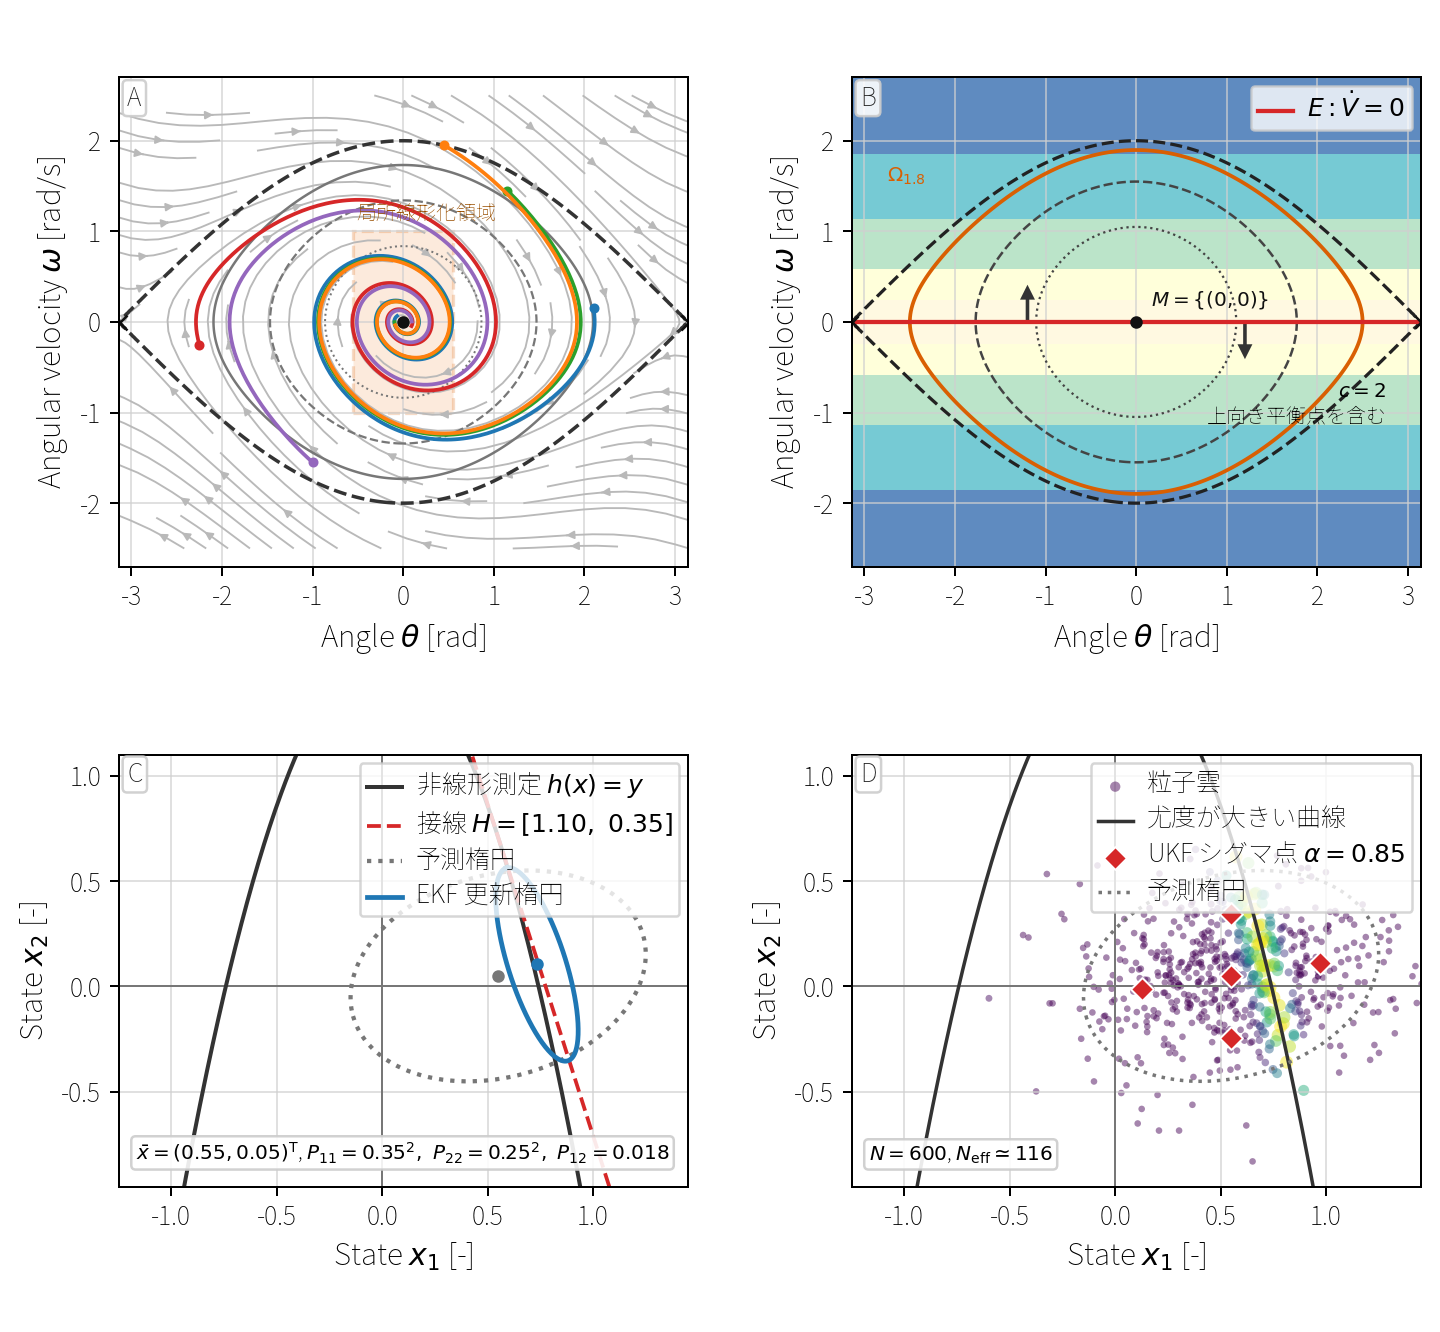
\includegraphics[width=0.95\linewidth,bb=0 0 1440 1332]{figures/nonlinear_geometry_estimation_examples.png}
\caption{非線形位相図、Lyapunov 準位集合、局所線形化領域、EKF の線形化楕円、UKF シグマ点、粒子雲の対応。上段は減衰係数 $0.35$ の正規化振子で、$V=2$ が上向き平衡点を通る境界になる。下段は $h(x)=x_1^2+0.35x_2$、$y=0.55$、$R=0.08^2$ の測定更新で、接線近似とサンプル表現の違いを示している。}
\label{fig:nonlinear-geometry-estimation-examples}
\end{figure}

図\ref{fig:nonlinear-geometry-estimation-examples}の数値は、局所近似と集合による判定を具体的に結び付けている。橙色の局所線形化領域の端である $\theta=0.55\,\mathrm{rad}$ では
\begin{equation}
  \frac{\abs{\sin 0.55-0.55}}{0.55}
  =
  \frac{\abs{0.5227-0.55}}{0.55}
  \simeq 4.97\times10^{-2}
\end{equation}
であり、小角近似 $\sin\theta\simeq\theta$ の相対誤差は約 $5.0\,\%$ である。この値は、橙色の長方形が「完全な線形領域」ではなく、数パーセント程度の曲率を許した局所モデルの作業領域であることを示す。エネルギー関数については
\begin{equation}
  V(\pi,0)
  =
  \frac{1}{2}0^2+1-\cos\pi
  =
  2
\end{equation}
となるため、$c=1.8$ の準位集合は上向き平衡点 $(\pi,0)$ を含まない。さらに $\dot{V}=0$ は $\omega=0$ の直線全体で成り立つが、その直線上で運動が止まり続けるには同時に $\dot{\omega}=-\sin\theta=0$ も必要である。したがって $c<2$ の内側で残る最大不変集合は下向き平衡点 $(0,0)$ だけであり、LaSalle の議論では $\dot{V}=0$ の集合そのものではなく、その中の最大不変集合を見る。

下段の測定写像でも、同じ局所化が接線として現れる。$h(x)=x_1^2+0.35x_2$ なので
\begin{equation}
  \left.\frac{\pp h}{\pp x}\right|_{\bar{x}}
  =
  \begin{bmatrix}
    2\bar{x}_1&0.35
  \end{bmatrix}
  =
  \begin{bmatrix}
    1.10&0.35
  \end{bmatrix}
\end{equation}
である。また、平均点での予測測定は $h(\bar{x})=0.55^2+0.35\cdot0.05=0.32$ であり、実測 $y=0.55$ との差は $0.23$ である。EKF はこの差を $H$ が張る接線方向の線形革新として扱うため、曲がった尤度集合を一つの楕円で表す。一方、UKF のシグマ点と粒子フィルタの粒子雲は、同じ測定曲線の曲率をサンプルの配置と重みに残す。
